\documentclass[a4paper]{article}
\usepackage[english]{babel}
\usepackage[utf8x]{inputenc}
% package for including graphics with figure-environment
\usepackage{graphicx}
% package for code blocks
\usepackage{listings}
% package for coloring code
\usepackage{xcolor}
\usepackage{hyperref}
% colors for hyperlinks
\hypersetup{colorlinks=true,citecolor=black,filecolor=black,linkcolor=black,urlcolor=black}
\lstdefinelanguage{Dafny}{
  morekeywords={method, function, predicate, var, const, type, ensures, requires, modifies, assert, 
  assume, if, then, else, while, new, class, datatype, trait, extends, ghost, reads, invariant, 
  writes, lemma, forall, exists, match, case, calc, returns, decreases, false, true},
  sensitive=true,
  morecomment=[l]{//},      % Single-line comments
  morecomment=[s]{/*}{*/},  % Multi-line comments
  morestring=[b]{"}         % Strings in double quotes
}
% Define Dafny listing style
\lstdefinestyle{dafnystyle}{
  language=Dafny,
  basicstyle=\ttfamily\footnotesize,
  keywordstyle=\color{blue}\bfseries,
  commentstyle=\color{gray}\itshape,
  stringstyle=\color{red},
  numbers=left,
  numberstyle=\tiny\color{gray},
  stepnumber=1,
  frame=single,             % Adds a border around the code block
  breaklines=true,          % Allows line breaking
  captionpos=b              % Caption position (bottom)
}


% package for bibliography
\usepackage[authoryear,round]{natbib}
% package for header
\usepackage[automark]{scrlayer-scrpage}
\pagestyle{scrheadings}
\ihead[]{Bogdan Kyuchukov}
\ohead[]{\today}
\cfoot[]{\pagemark} 
\setheadsepline[122mm]{0.3mm}
\begin{document}
\title{
	\vspace{1cm}
	\Huge Verifying imperative programs \\ with Dafny \\
}

\vspace{1cm}

% Insert here your name and correct mail address
\author{\Large \href{mailto:B.Kyuchukov@campus.lmu.de}{Bogdan Kyuchukov}
	\vspace{1cm}}

% name of the course and module
\date{
	\large Ludwig Maximilian University of Munich \\ Course: Deductive Software Verification \\
	\vspace{0.8cm}
	\large Lecturer: Prof. Gidon Ernst\\
	\vspace{1cm}
	\today
}

\maketitle
\setlength{\parindent}{0pt}

\vspace{2cm}
\begin{abstract}
	The goal of this work is to show how to formally reason
	about imperative programming constructs such as
	loops, arrays and dynamically allocated objects. To be able to achieve that, basic
	Dafny constructs will be shown, such as functions, methods, pre- and postconditions. The discussion thereafter will move
	towards recursion and termination as well as inductive datatypes. Having learned from those chapters,
	loop invariants and their usage will be explored. Because analyzing objects in the heap is more challenging,
	searching and modifying arrays will be covered. The final chapter will include a detailed discussion about Dafny's
	dynamic frames and their significance.
\end{abstract}
\newpage
\tableofcontents
\newpage

\section{Introduction}
\label{sec:introduction}
\subsection{Why Dafny?}
When software engineers encounter the field of formal methods and verification, this usually happens
in an academic setting, where proof techniques are learned and done by hand. Moreover, actually taking advantage
of those methods in practice involves a steep learning curve and lots of time. This unfortunately leads to less
acceptance of verification techniques in
an industry where fast time to market is essential \cite{reid2020makingformalmethodsnormal}. Dafny promises to solve those problems. As a programming
language designed to support specifications and proofs, it comes with an automated verifier that integrates
seamlessly into most modern IDEs \footnote{Integrated Development Environments (IDEs)} making rigorous verification part of the software development process,
thus reducing costly late-stage bugs that may be missed by testing. The language was designed by Rustan Leino in
2009 and it's current version at the time of this writing is 4.9.0 from 31. October 2024. Dafny is heavily
used at Amazon Web Services to develop critical components of their access management, storage, and cryptography infrastructures \cite{Chakarov2022}.

\subsection{Dafny's build system}
The main idea in such verification-aware programming languages is that code is divided into two parts - the
specification part and the implementation part \cite{leino2023program}. The built-in verifier in Dafny acts as an
extended type checker and constantly proves that the provided implementation actually meets the behavior stated in
the specification part of the given function, method or class. This is done by transforming the code into an intermediary
that a tool called Boogie can understand. The correctness of the Boogie program implies the correctness of the
Dafny program. Boogie then generates first-order verification rules that are passed to the
Z3 SMT solver. Any violations of these conditions are passed back as verification errors \cite{Herbert2012}. Apart
from C\#, Dafny can be compiled to many other programming languages. This process is visualized in
Figure \ref{fig:build-system}.
\begin{figure}[h]
	\centering
	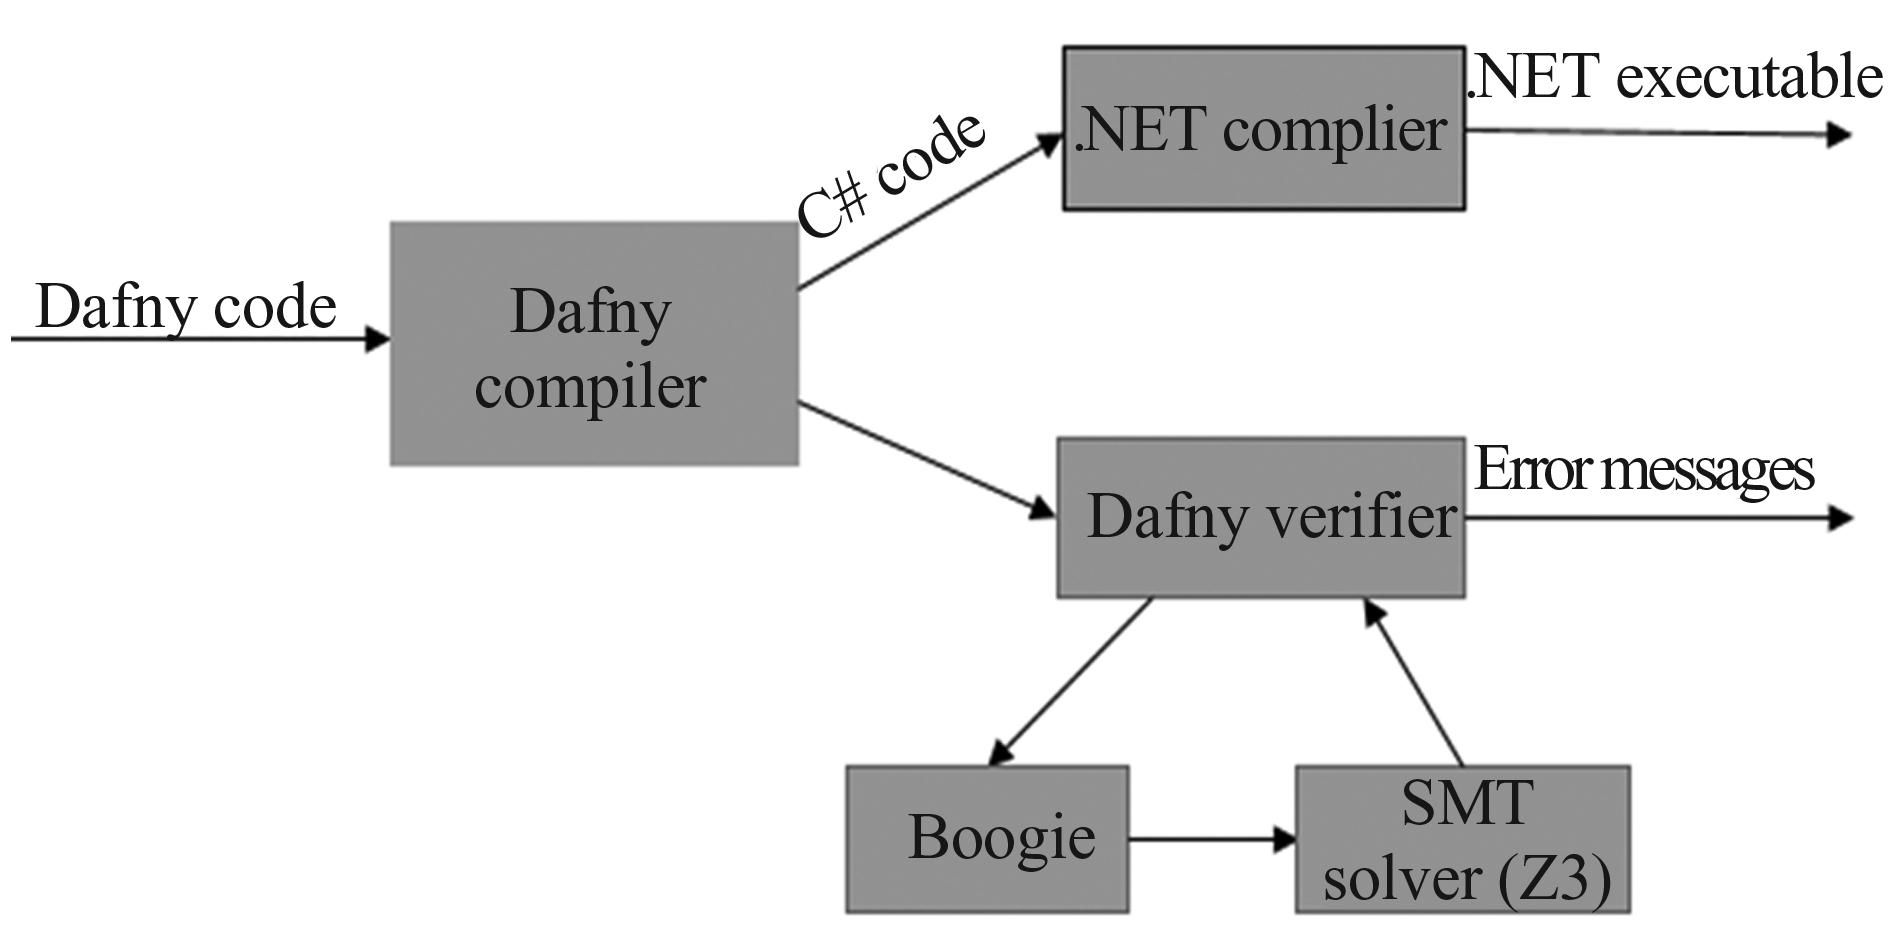
\includegraphics[width=0.80\textwidth]{images/dafny-infra.jpg}
	\caption{The Dafny build system as shown in \cite{Herbert2012}}
	\label{fig:build-system}
\end{figure}
% Dynamic Frames
\section{Building Blocks of Dafny}
\label{sec:foundations}
This work assumes the reader is familiarized with the fundamentals of program-semantics such as Floyd logic and
Hoare triples, as they build the reasoning framework of Dafny and help to understand it more effectively.

\subsection{Methods}
As in other programming languages, a \textit{method} is a block of code that prescribes some behavior. For instance,
Listing \ref{lst:dafnymethod} shows the declaration of a method called \texttt{Triple}.
\begin{lstlisting}[style=dafnystyle, caption={Simple method in Dafny.}, label={lst:dafnymethod}]
method Triple(x: int) returns (r: int)
 ensures Average(x) == 3 * x {
  var y := 3 * x;
  r := x + y;
}
\end{lstlisting}
This method takes an \textit{in-parameter} x of type integer and returns an \textit{out-parameter} r, also
of type integer. The \textbf{ensures} keyword is used to specify the method's \textit{postcondition}. A postcondition expresses a property
that must hold after every invocation of the method through all possible return points.
Postconditions are part of the method's specification and appear before the body block \cite{Herbert2012}.
The body of a method is a list of statements that give the method's implementation. In Dafny,
methods can have any number of in- and out-parameters. Inside the method, the out-parameters are like local
variables and can be assigned and read. When the method ends, whatever values were assigned to the out-parameters
will be returned to the caller. The in-parameters however cannot be re-assigned \cite{leino2023program}.

\subsection{Functions}
Functions in Dafny are very mathematical in nature, because they are deterministic. Any two invocations of a
function with the same arguments will result in the same value. Listing \ref{lst:dafnyfunction} shows how a simple
function named \texttt{Average} looks like.
\begin{lstlisting}[style=dafnystyle, caption={Simple function in Dafny.}, label={lst:dafnyfunction}]
function Average(a: int, b: int): int 
 requires 0 <= a && 0 <= b {
  (a + b) / 2
}
\end{lstlisting}
Whereas a method is declared to have some number of out-parameters, a function instead declares a result type,
and while a method body is a statement, the body of a function is an expression \cite{leino2023program}.
Another important difference between functions and methods is, that functions are \textit{transparent}. This means
that their implementation is directly visible to the caller. That's the reason why functions can also be used
to describe pre- and postconditions like the precondition on line 2 in Listing \ref{lst:dafnyfunction}.
Methods on the other hand are \textit{opaque}, so callers fully rely on the postcondition to reason about their return values.
\subsection{Ghost constructs}
Sometimes when reasoning about a program more information is needed than what the compiler has at runtime.
A declaration, variable, statement, etc., that is used only for specification purposes is called a \textit{ghost}.
The verifier takes all ghosts into account, whereas the compiler erases all ghosts when it produces executable code.
Other ghost constructs include pre- and postconditions (declared by \textbf{requires} and \textbf{ensures} clauses).
They are used solely to specify the behavior of the program and establish a contract between callers and implementations \cite{leino2023program}.
\begin{lstlisting}[style=dafnystyle, caption={Invalid assignment to ghost.}, label={lst:dafnyghost}]
method InvalidAssignment() returns (y: int) {
  ghost var x := 10;
  y := 2 * x; // cannot assign to compiled variable using a ghost
}
\end{lstlisting}
To make sure ghost constructs can be successfully deleted after compilation, Dafny makes sure the compiled code
doesn't rely on any ghost constructs. Listing \ref{lst:dafnyghost} demonstrates a violation of this rule, which
results in a verification error.

\section{Recursion and termination}
A recursive function is one that calls itself directly or indirectly. To be able to terminate, all recursive
functions need a base case - a condition where the function stops calling itself and returns a result. An example
is shown with a function called \texttt{SeqSum} in Listing \ref{lst:dafnyrec}, which computes the sum of all
integers in a sequence. On line 4, if the base case isn't met, the function invokes itself with an incremented value for lo.
\begin{lstlisting}[style=dafnystyle, caption={Function computing the sum of all integers in a sequence recursively.}, label={lst:dafnyrec}]
function SeqSum(s: seq<int>, lo: int, hi: int): int
  requires 0 <= lo <= hi <= |s|
  decreases hi - lo {
  if lo == hi then 0 else s[lo] + SeqSum(s, lo + 1, hi)
}
\end{lstlisting}
\subsection{The decreases clause}
Dafny can prove termination by using the \textbf{decreases} clause. If we can label each function invocation with
a natural number and make sure that successive invocations strictly decrease that label, then it follows
that at run time the recursive calls can only execute a finite number of times, and that is all the information
needed to prove that the recursion eventually terminates \cite{Herbert2012}. As shown on line 3 in Listing
\ref{lst:dafnyrec}, the label of each invocation of \texttt{SeqSum} decreases gradually, because with each invocation
the difference between hi and lo is smaller. When it reaches zero, the recursion terminates.
\subsection{Well-founded relations}
Termination metrics are not restricted to natural numbers.
Termination can also be proven when two labels, which represent successive recursive invocations, are in a relation
that is \textit{well-founded} \cite{leino2023program}. This relation, denoted as $a \succ b$, signifies that a
reduces to b. For it to be \textit{well-founded}, the following three conditions must be true:
\begin{itemize}
	\item $ \succ $ is \textit{reflexive}: The relation never relates an element to itself. $a \succ a$ never holds.
	\item $ \succ $ is \textit{transitive}: Whenever $a \succ b$ and $b \succ c$ hold, then so does $a \succ c$.
	\item $ \succ $ satisfies the \textit{descending chain condition}: the relation has no \textit{infinite descending chain}.
\end{itemize}
From these conditions it follows that a well-founded relation is a strict partial order that additionally
satisfies the descending chain condition. Dafny pre-defines $ \succ $ for each data type, and in some cases also
for values between different types (but in most cases, values from different types are not related in
this partial order) \cite{leino2023program}.

\section{Inductive datatypes}
In order to accomplish meaningful tasks, programs need to define their own data structures. A useful way to do that
is to use \textit{datatypes}. They define what \textit{variants} data can have and what \textit{payload} each variant
carries. In contrast to classes, which describe mutable \textit{state}, datatypes describe immutable \textit{values}
\cite{leino2023program}. Datatypes are often defined recursively. That is, values can be built up from simple
variants or from variants that contain other datatypes. For this reason, they are known as \textit{inductive datatypes}
\cite{leino2023program}.
\begin{lstlisting}[style=dafnystyle, caption={A simple and an inductive datatype.}, label={lst:dafnydatatype}]
// enumeration
datatype Color = White | Yellow | Blue | Red

// inductive datatype, parameterized
datatype Tree<T> = Leaf(data: T) | 
		Node(left: Tree<T>, right: Tree<T>)
\end{lstlisting}
The type \texttt{Tree<T>} shown in Listing \ref{lst:dafnydatatype} can be parameterized with the type of its payload,
that is, the data stored in the tree. One can also define functions on datatypes.
\begin{lstlisting}[style=dafnystyle, caption={Function defined on a datatype.}, label={lst:dafnydatafun}]
function Size<T>(t: Tree<T>): nat {
  match t
  case Leaf(_) => 1
  case Node(left, right) => Size(left) + Size(right)
}
\end{lstlisting}
Listing \ref{lst:dafnydatafun} shows a function \texttt{Size}, parameterized by a type \texttt{T} and a value t of type
\texttt{Tree<T>}, that returns the number of leaf nodes in t. When calling a function, the type arguments can
usually be inferred. If so, as seen on line 4 in Listing \ref{lst:dafnydatafun}, we can omit them
(along with the angle brackets) \cite{leino2023program}.
\subsection{Discriminators and destructors}
Very often when working with datatypes, there is a need to know the variant of the datatype value. That is, to know
which constructor was used to create the value. One could write a function like the one shown in Listing \ref{lst:dafnydatapred}
that determines this.
\begin{lstlisting}[style=dafnystyle, caption={Predicate checking if the argument t is a Node.}, label={lst:dafnydatapred}]
predicate IsNode(t: Tree<T>) {
  match t
  case Leaf(_) => false
  case Node(_, _) => true
}
\end{lstlisting}
Because this is such a common operation, Dafny pre-defines such a \textit{descriminator} for each constructor.
The name of the discriminator is the name of the constructor followed by a question mark as shown on line 2
in Listing \ref{lst:dafnydatadiscr}.
\begin{lstlisting}[style=dafnystyle, caption={Function returning the left subtree of a tree.}, label={lst:dafnydatadiscr}]
function GetLeft(t: Tree<T>): Tree<T>
 requires t.Node? {
  match t
  case Node(left, _) => left
}
\end{lstlisting}
The discriminators are \textit{members} of the type, which means they are accessed by following an expression with a dot
and the name of the member \cite{leino2023program}. The precondition of \texttt{GetLeft} says the function can only be
applied to a tree of the \texttt{Node} variant. This means that the \texttt{match} expression only needs to consider
one case. Because \texttt{GetLeft} is also a common operation, Dafny provides a convenient way to declare such a
\textit{destructor} for each parameter of the constructor. This is done by simply naming the parameter \cite{leino2023program}.
Line 6 in Listing \ref{lst:dafnydatatype} demonstrates this with the parameters \texttt{left} and \texttt{right}.
Because destructors are also members of the type, they can be accessed the same way as discriminators.

\section{Loop invariants}
Many interesting computations are described as repetitions of steps. Apart from recursion,
the other way of repeating code is the \textit{loop}. The main way to reason about any loop is the
\textit{loop invariant}. It's part of the loop specification and restricts the state space that the loop is
allowed to explore \cite{leino2023program}. Another key component is the \textit{loop guard}, which controls
whether the loop continues to perform steps or it stops doing so.
\begin{lstlisting}[style=dafnystyle, caption={Simple while loop.}, label={lst:dafnyloop}]
i := 0;
while i < 100
 // decrease 100 - i is added implicitly
 invariant 0 <= i <= 100 {
 i := i + 1;
}
assert i == 100; // true
\end{lstlisting}
In the example shown in Listing \ref{lst:dafnyloop} the loop guard is the condition of the while loop on line 2. The
loop invariant is defined on line 3 and specifies that i is only allowed to be in the range between 0 and 100. It's
important that, on entry to the loop, both the loop invariant and the loop guard hold. On exit from the loop, only
the loop invariant holds. The loop guard is negated. When working with loops, it's a good practice to make the loop
invariant as restrictive as possible in order to have a clear specification of what needs to happen inside the loop.
\subsection{Binary search}
To effectively illustrate the advantages of Dafny, we will analyze the implementation of the binary search
algorithm and provide a detailed discussion of each step. In this context,
loop invariants play a crucial role.
\subsubsection{Precondition}
Binary search requires the array it searches to be sorted. Listing \ref{lst:dafnybinaryprecond}
specifies this precondition with the help of the universal quantifier.
\begin{lstlisting}[style=dafnystyle, caption={All elements of array \texttt{a} are sorted.}, label={lst:dafnybinaryprecond}]
forall i, j :: 0 <= i < j < a.Length ==> a[i] <= a[j]
\end{lstlisting}
It says that if we take two indices into the array, i and j where i is placed to the left of j,
then the elements at those two indices are ordered properly. The operator \texttt{==>} means implication, i.e.
if the condition on its left side holds, then the condition to its right side must also hold.
\subsubsection{Postconditions}
To begin with, the caller has to be assured that the returned index is inside the array bounds. Line 3 in Listing
\ref{lst:dafnybinarypostcond} specifies this. If the element we search for exists in the array, we want to
return the index of its leftmost occurrence. Otherwise we want to return its earliest insertion point.
The specification has to ensure that all elements in the array that appear before the element at the returned
index must be smaller than it, as shown on line 4 in Listing \ref{lst:dafnybinarypostcond}. Similarly,
all elements that appear after it must be greater than or equal to it,
as indicated on line 5 of Listing \ref{lst:dafnybinarypostcond}.
\begin{lstlisting}[style=dafnystyle, caption={Binary search pre- and postconditions.}, label={lst:dafnybinarypostcond}]
method BinarySearch(a: array<int>, key: int) returns (n: int)
  requires forall i, j :: 0 <= i < j < a.Length ==> a[i] <= a[j]
  ensures 0 <= n <= a.Length
  ensures forall i :: 0 <= i < n ==> a[i] < key
  ensures forall i :: n <= i < a.Length ==> key <= a[i]
\end{lstlisting}
\subsubsection{Missing loop invariants}
The main idea of binary search is that we have two indices, lo and hi, that form a window inside the array. Anything
to the left of the window is too small to be our element and anything to the right is at least as large. This
window keeps shrinking until it reaches 0, at which point both lo and hi meet. A logarithmic number of iterations is
obtained by halving the window with each time. Part of the implementation is shown in Listing \ref{lst:dafnybinarypartimpl}.
\begin{lstlisting}[style=dafnystyle, caption={Binary search implementation with verifier errors.}, label={lst:dafnybinarypartimpl}]
// Error: A postcondition couldn't be proved on this return path.
var lo, hi := 0, a.Length;
while lo < hi {
  var mid := (lo + hi) / 2;
  if a[mid] < key { // Error: index out of range.
    lo := mid + 1;
  } else {
    hi := mid;
  }
}
\end{lstlisting}
An essential part of the implementation is missing in Listing \ref{lst:dafnybinarypartimpl}, namely the loop
invariants. Since the loop guard on line 3 holds, we enter the loop, but the automated verifier reports an error on
line 5, because there is no loop invariant to bind the integer state space of lo and hi to be
between 0 and \texttt{a.Length} respectively. Furthermore, the verifier reports another error directly at the
beginning of the method, because the postconditions formulated on lines 4 and 5 in Listing \ref{lst:dafnybinarypostcond}
are not guaranteed to hold neither during, nor after the loop.
\subsubsection{Adding loop invariants}
There exists a very neat, refined design technique
for loop specifications called "Replace Constant By Loop Variable" described in detail in \cite{leino2023program}.
Basically, it says you can take your desired postconditions, copy them to use as loop invariants, and then simply
swap out their constant, in this case n, for the loop index, in this case both lo and hi. Listing
\ref{lst:dafnybinaryfullimpl} demonstrates these changes.
\begin{lstlisting}[style=dafnystyle, caption={Binary search implementation withiout verifier errors.}, label={lst:dafnybinaryfullimpl}]
{
  var lo, hi := 0, a.Length;
  while lo < hi
  invariant 0 <= lo <= hi <= a.Length
  invariant forall i :: 0 <= i < lo ==> a[i] < key
  invariant forall i :: hi <= i < a.Length ==> key <= a[i] {
    var mid := (lo + hi) / 2;
    if a[mid] < key {
      lo := mid + 1;
    } else {
      hi := mid;
    }
  }
  n := lo;
}
\end{lstlisting}
Finally, the added loop invariants ensure correctness at each loop iteration and establish the postconditions
afterwards. The whole \texttt{BinarySearch} method is a combination of both Listing \ref{lst:dafnybinarypostcond}
and Listing \ref{lst:dafnybinaryfullimpl}.

\section{Arrays and simple frames}


\section{Classes and dynamic frames}


\newpage

\listoffigures
\lstlistoflistings
\bibliographystyle{apalike}
\bibliography{references}
\addcontentsline{toc}{section}{References}
\end{document}